\documentclass{article}
\usepackage{graphicx} % Required for inserting images

\title{《电子电路基础》课程设计报告}
\author{}
\date{2025年12月12日}
\usepackage[UTF8]{ctex}
\usepackage{graphicx}

\usepackage{ulem}
\usepackage{enumitem}
\usepackage{titlesec}
\usepackage{multicol}
\usepackage[export]{adjustbox}
\usepackage{amsmath}  % 推荐用于更好的数学排版
\usepackage[utf8]{inputenc}
\usepackage{CJKutf8}
\usepackage{fancyhdr}
\usepackage{lastpage}
\usepackage{ulem}
\usepackage{tabularx}
\usepackage{float}

\usepackage{pgfplots}
\usepackage{float}
\usepackage{tikz}
\usepackage{ctex}
\usepackage{geometry}
\usepackage{color}
\usepackage{pgfplots}
\geometry{a4paper}
\geometry{left=2cm} 
\geometry{right=2cm} 
\geometry{top=2cm} 
\geometry{bottom=2cm} 
\linespread{1.5}%

\begin{document}

\maketitle

\section*{1 设计运算放大器}

\textbf{要求}

现有双极型晶体管 $\beta = 100$,$V_T=26\text{mV}$，可采用理想电流源，请设计一款运算放大器，满足以下条件：

（1）电压放大倍数 $\geq 60\mathrm{dB}$；（2）输入电阻 $\geq 100\mathrm{k}\Omega$；（3）输出电阻 $\leq 100\Omega$

请推导出你所设计的电路电压放大倍数、输入电阻和输出电阻的详细计算公式，检查其是否满足以上设计目标。

\textbf{分析}

运算放大器一定需要一个差分放大电路，然后根据增益要求需要多级放大电路，同时针对输入输出电阻的要求，其中也需要加入射级跟随器。因此，我们可以设计如下电路：

\begin{figure}[H]
\centering
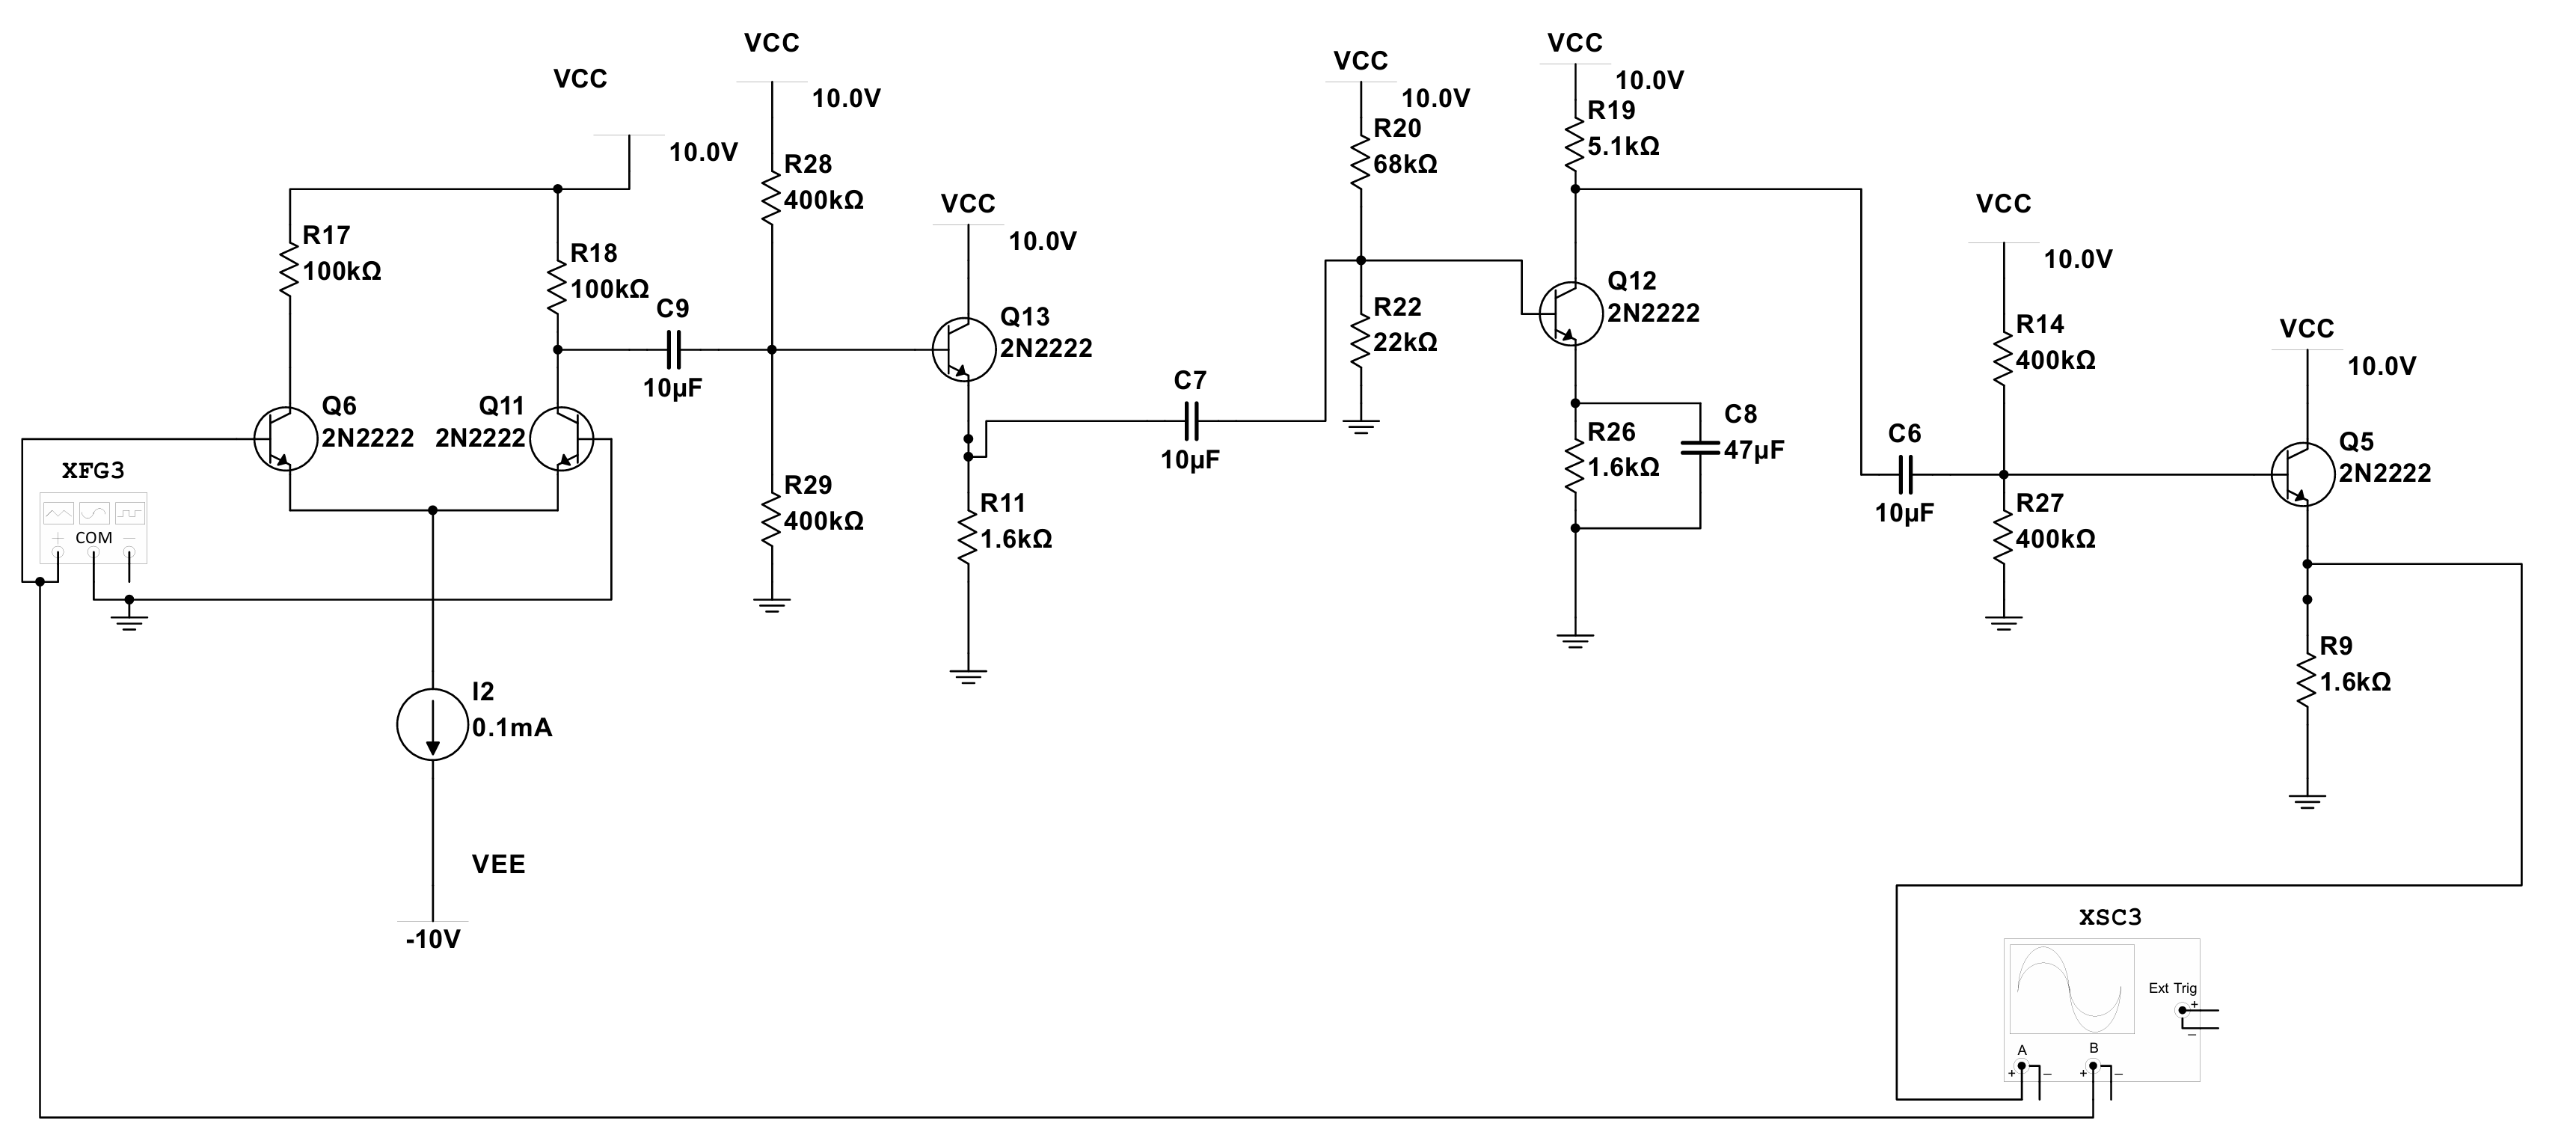
\includegraphics[width=0.8\textwidth]{1.png}
\caption{运算放大器整体电路}
\end{figure}

如图所示，整个电路依次由一个差分放大电路、一个射极跟随器、一个共射级放大电路和另一个射极跟随器组成。下面我们将分模块推导各个电路的电压放大倍数、输入电阻和输出电阻。由于下一级电路的输入电阻会作为前一级电路的负载从而影响放大倍数，我们将从后向前分析。


\subsection*{1.1 射极跟随器(1)}

\begin{figure}[H]
\centering
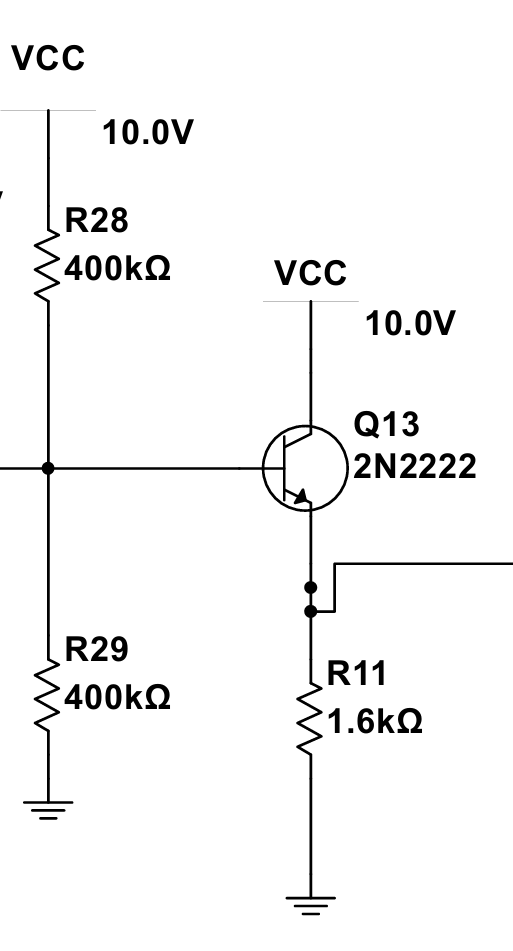
\includegraphics[width=0.2\textwidth]{3.png}
\caption{射极跟随器电路}
\end{figure}

\textbf{直流分析}

戴维南等效\[V_{Th}=5\text{V},R_{Th}=200\text{k}\Omega \]

由\[V_{Th}-\frac{I_C}{\beta}R_{Th}-0.7-I_CR_E=0\]

解得\[I_C=1.194\text{mA} \]

\textbf{交流分析}

be结动态电阻\[r_{be}=\beta \frac{V_T}{I_C}=2.178\text{k}\Omega \]

放大倍数\[ A_u=\frac{1}{1+\frac{r_{be}}{(1+\beta)(R_C//R_L)}}\approx 1\]

输出电阻\[R_o=R_e//\frac{r_{be}}{1+\beta}=21.275\text{k}\Omega<100\text{k}\Omega \]

\textbf{输出电阻满足设计要求。}

输入电阻\[R_i=[r_{be}+(1+\beta)(R_E//R_L)]//(R_B/2) \]

最后一级输出空载，\(R_L=0\), 所以\[R_i=90.04\text{k}\Omega \]

\subsection*{1.2 共射级放大电路}

\begin{figure}[H]
\centering
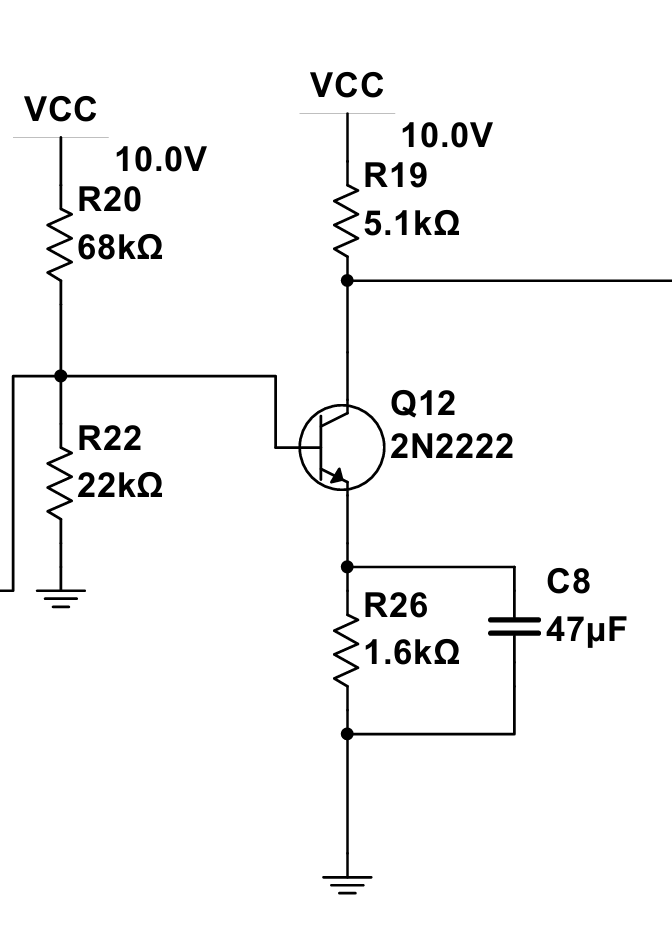
\includegraphics[width=0.2\textwidth]{4.png}
\caption{共射级放大电路}
\end{figure}

\textbf{直流分析}

戴维南等效\[V_{Th}=2.44\text{V},R_{Th}=16.62\text{k}\Omega \]

由\[V_{Th}-\frac{I_C}{\beta}R_{Th}-0.7-I_CR_E=0\]

解得\[I_C=0.987\text{mA} \]

\textbf{交流分析}

be结动态电阻\[r_{be}=\beta \frac{V_T}{I_C}=2.634\text{k}\Omega \]

将下一级输入电阻代入负载阻值，算得放大倍数\[ A_u=\frac{(1+\beta)(R_C//R_L)}{R_{B1}//R_{B2}//r_{be}}=214.29\]

输入电阻\[R_i=R_{B1}//R_{B2}//r_{be}=2.274\text{k}\Omega \]

\subsection*{1.3 射极跟随器(2)}



\textbf{交流分析}

和刚才的射极跟随器同理，放大倍数仍为\( A_u\approx 1\)，但负载为下一级的输入电阻，\(R_L=R_i\), 所以这一级的输入电阻\[R_i=65.34\text{k}\Omega \]





\subsection*{1.4 差分放大电路}

\begin{figure}[H]
\centering
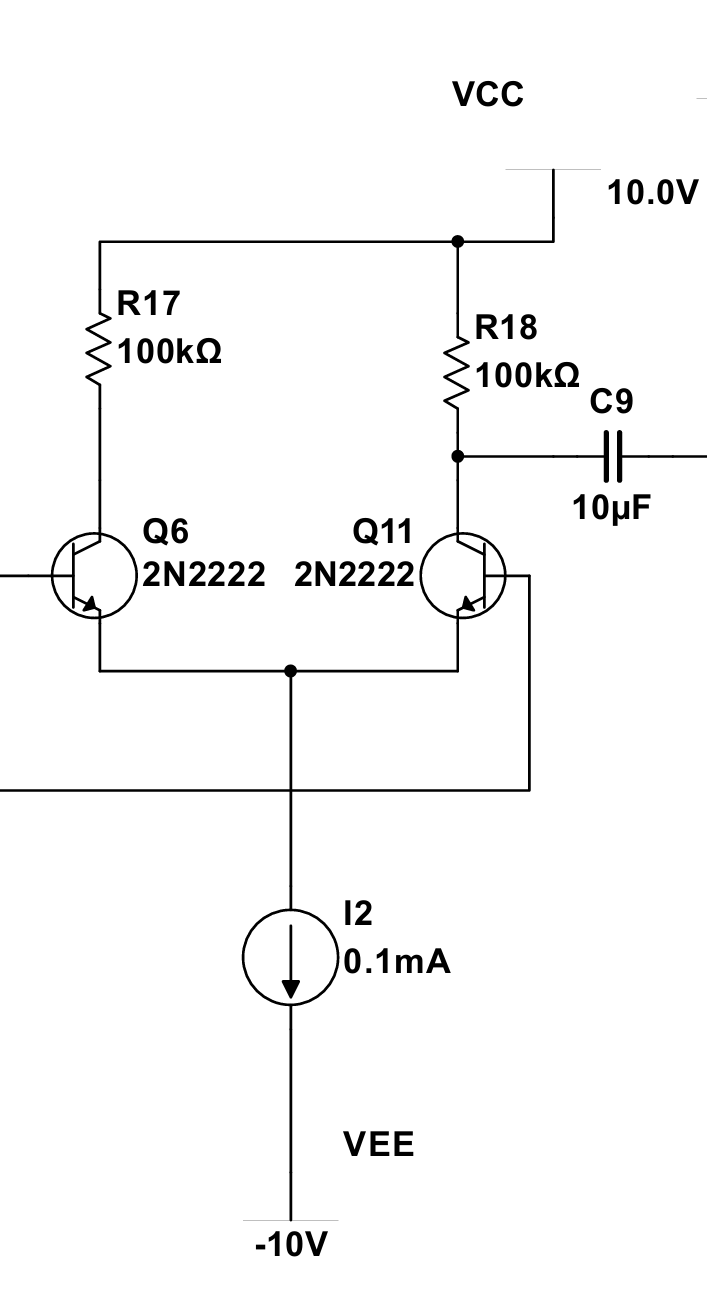
\includegraphics[width=0.2\textwidth]{2.png}
\caption{差分放大电路}
\end{figure}


be结动态电阻\[r_{be}=\beta \frac{V_T}{I_C}=52\text{k}\Omega \]

输入电阻\[R_i=2r_{be}=104\text{k}\Omega>100\text{k}\Omega \]

\textbf{输入电阻满足设计要求。}

差模增益\[A_d=-\frac{\beta(R_C//R_L)}{2r_{be}}=38.0\]

总增益\[A_u=38.0\cdot 214.29=8143.02=78.216\text{dB}>60\text{dB} \]

\textbf{电压放大倍数满足设计要求。}

\textbf{仿真}

使用Multisim软件进行仿真，输入0.1mVpp正弦波，得到输入输出波形：

\begin{figure}[H]
\centering
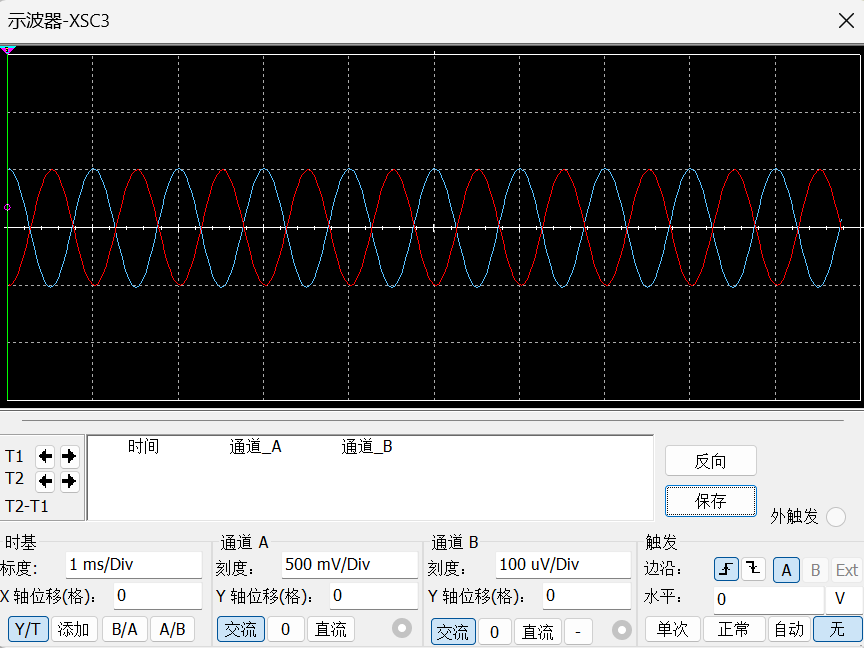
\includegraphics[width=0.4\textwidth]{5.png}
\caption{输入输出波形}
\end{figure}

可以粗略看出放大倍数为5000，虽与理论值有一定差距，但仍旧满足设计目标。

\section*{2 设计运算电路}

\textbf{要求}

利用理想运算放大器，设计满足下面计算公式的电路：
\[
V_{\text{out}} = \sum_{i=1}^4 a_i v_i
\text{,其中}a_i = [-1.5,\; -0.5,\; 1.5,\; 0.5]\]

请尽量减少运算放大器的使用数量。

\textbf{分析}

计算公式的系数有正有负，有大于1的，也有小于1的。如果使用同相加法器，只能实现放大而不能实现缩小。若使用双端输入式求和电路，虽然只需要用到一个理想运放，但系数调节是非常困难的。

\begin{figure}[H]
\centering

\includegraphics[width=0.4\textwidth]{6.png}
\caption{双端输入式求和电路}
\end{figure}

\[
v_O = -\frac{R_5}{R_1} v_{S1} 
   - \frac{R_5}{R_2} v_{S2} 
   + \left( 1 + \frac{R_5}{R_1 // R_2} \right) 
     \left( 
         \frac{R_4}{R_3 + R_4} v_{S3} 
         + \frac{R_3}{R_3 + R_4} v_{S4} 
     \right)
\]

不如对公式变形
\[V_O=-1.5V_1-0.5V_2+1.5V_3+0.5V_4=-1.5V_1-0.5V_2-(-1.5V_3-0.5V_4)\]

这样用两个反向加法器级联便可实现计算公式。最终电路图如下：

\begin{figure}[H]
\centering

\includegraphics[width=0.5\textwidth]{7.png}
\caption{最终运算电路}
\end{figure}

\textbf{仿真}

使用Multisim软件进行仿真，在四个输入端输入不同幅值的正弦信号，其中
\[V_1=1.3\text{V},V_2=2.7\text{V},V_3=0.9\text{V},V_4=1.4\text{V}\]

\begin{figure}[H]
\centering

\includegraphics[width=0.6\textwidth]{8.png}
\caption{仿真结果}
\end{figure}

则计算公式和仿真结果一致，输出电压为
\[V_o=-1.25\text{V}\]
负号表示输出与输入反相。\textbf{运算电路满足设计要求。}

\begin{figure}[H]
  \centering
  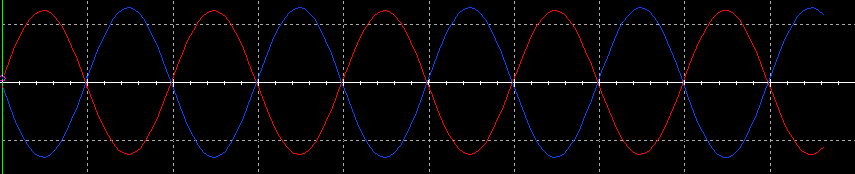
\includegraphics[width=0.6\textwidth]{9.png}
  \caption{输出与输入反相}  
\end{figure}



\section*{3 分析}

\textbf{问题}

如果将理想运算放大器替换为你所设计的放大器，上一部分中所构成的函数会发生什么改变？

\textbf{分析}

理想运放的假设条件是：
\begin{itemize}
    \item 开环增益无穷大
    \item 输入电阻无穷大
    \item 输出电阻为零
    \item 共模抑制比无穷大
    \item 无失调电压/电流
\end{itemize}

我们设计的放大器的实际参数是：
\begin{itemize}
    \item \textbf{有限的开环增益}：我们刚才设计出的“运算放大器”是一个具体的晶体管多级放大器，其电压放大倍数 \(A_v\) 是有限的（\(\geq 1000\) 倍，即 \(60\ \text{dB}\)）。  
    在求和电路中，如果它是用来构成反相求和或同相求和电路，则闭环增益取决于外部电阻匹配与运放的开环增益大小。  
    如果实际 \(A_{v0}\) 有限，则闭环增益公式  
    \[
    A_{f} \approx \frac{A_{v0}}{1 + A_{v0} \beta}
    \]  
    中的 \(\beta\) 是反馈系数。理想情况下 \(A_f = 1/\beta\)，但有限 \(A_{v0}\) 时实际增益会略小于理想值，并且与频率有关。

    \item \textbf{输入电阻非无穷大}：  
    我们设计的运算放大器的输入电阻 \(R_{\text{in}} \geq 100\ \text{k}\Omega\)，而理想运放输入电阻无穷大。  
    在反相加法器中，实际运放的输入电阻有限会影响输入端的电流分配，使求和系数产生误差。  
    在同相加法器中，有限输入电阻会改变电压分压关系，导致系数不准确。

    \item \textbf{输出电阻非零}：  
    我们设计的运算放大器的输出电阻 \(R_{\text{out}} \leq 100\ \Omega\)，理想运放输出电阻为零。  
    实际运放输出电阻会在负载变化时引起输出电压变动，当负载较重或反馈网络吸收电流时，输出可能达不到理论值。

    \item \textbf{失调与温漂}：  
    晶体管实际运放存在输入失调电压 \(V_{\text{os}}\)、输入失调电流 \(I_{\text{os}}\)，这会使得在 \(v_i = 0\) 时 \(V_{\text{out}} \neq 0\)，并且系数实现时叠加了直流误差。

    \item \textbf{带宽限制}：  
    我们设计的晶体管运放有有限的增益带宽积，当信号频率较高时，各通道的增益会下降且可能产生相移，对于多路信号叠加可能引入频率相关误差。
\end{itemize}

因此，原来理想的线性运算电路变成了一个受实际运放参数限制的近似运算电路。

\end{document}